
%(BEGIN_QUESTION)
% Copyright 2010, Tony R. Kuphaldt, released under the Creative Commons Attribution License (v 1.0)
% This means you may do almost anything with this work of mine, so long as you give me proper credit

Explain how you would use a multimeter (and any other appropriate electronic test equipment) to test the following components of a passive (zener) IS barrier module.  For each test, identify both the multimeter setting and the connection points for the multimeter's test leads (A, B, C, D; red, black), as well as the reading expected if the component in question is good.

$$\includegraphics[width=15.5cm]{i02516x01.eps}$$

\begin{itemize}
\item{} How to test for proper zener breakdown voltage:
\vskip 100pt
\item{} How to check for a shorted zener diode:
\vskip 100pt
\item{} How to check for a good fuse:
\end{itemize}

\vfil

\underbar{file i02516}
\eject
%(END_QUESTION)





%(BEGIN_ANSWER)

This is a graded question -- no answers or hints given!

%(END_ANSWER)





%(BEGIN_NOTES)

\noindent
{\bf How to test for proper zener breakdown voltage:}

The principles to keep in mind here are that zener diodes break down when reverse-biased, and that the current passing through them during breakdown must be limited in order to avoid damaging the diode.  

Connect a DC power supply slightly greater than 24 VDC to terminals A (+) and B ($-$), reading voltage at terminals C and D.  The voltmeter should read 24 VDC, even as the power supply voltage is increased.

\vskip 20pt

\noindent
{\bf How to check for a shorted zener diode:}

The principle here is that any shorted component will exhibit a much lower electrical resistance that it normally would.

An ohmmeter connected between terminals A and B (both polarities) should read ``open'' if no zener diode is shorted.  The same test applied between terminals C and D is not recommended, as a blown fuse would produce the same reading even with shorted diodes.

\vskip 20pt

\noindent
{\bf How to check for a good fuse:}

In order to check any device for continuity, we must pass a test current through that device.  An ohmmeter connected between terminals A and C (any polarity) should register the resistance of the resistor: 200 ohms.

%INDEX% Safety, intrinsic: passive zener barrier circuit

%(END_NOTES)


